\chapter{Use case: Next order prediction} \label{chapter:use-case}

One of the goals of this project is to integrate an artificial intelligence solution within a CRM. Based on the research reported in chapter \textit{CRM AI}, it has been decided to develop a predictive machine learning model with real world data from a CRM. This part of the thesis has been developed in collaboration with one of ELCA's client, hereafter referenced as \textit{Contoso} \footnote{Client's name and business subject to confidentiality.}.

This chapter details the entire machine learning project. Sections \ref{sec:use-case} and \ref{sec:ml-metrics} explain the business problem \textit{Contoso} is facing and how a machine learning solution might solve it. The data contained in Contoso's CRM is reported in section \ref{sec:crm-data} and section \ref{sec:ml-experimentation} details the machine learning experimentations. The model's deployment and integration within Contoso's CRM are outlined in section \ref{sec:crm-deployment}. Finally, sections \ref{sec:use-case-further-work} and \ref{sec:use-case-conclusion} conclude the chapter with a reflection on the entire initiative.

% -------------------------------- Section: Client's use case
\section{Client's use case} \label{sec:use-case}
\textit{Contoso} is an energy-focus company active overall Switzerland. Among the offers and services, Contoso's key-product is subject to a very tense market, where its characteristics are the same among all competitors and the price is the only differentiator. When dealing with this product, several of its specificities must be considered:
\begin{itemize}
\item The product is classified as a \textit{safety need} in Maslow's \textit{hierarchy of }needs\cite{wiki:Maslow's_hierarchy_of_needs}. People buy the product because they \textit{need} it and not because they \textit{like} it.
\item Due to its classification in Maslow's hierarchy, the product is usually stored in high quantities. The typical customer will make a large order, fill its supplies, consume the product and once fully consumed, the product is bought again in large quantities. Therefore, the product is not bought on a daily or weekly basis but rather on an annual basis. This is a real difficulty for Contoso while trying to build customer loyalty.
\item Since product's characteristics are the same for the entire market, the price is the only variable that companies can \textit{play} with. Nevertheless, part of the price is subject to global market variations, from which companies will adapt their margins. As all stock market, the prices can vary, even marginally, each day.
\end{itemize}

 Based on these particularities, building a solid customer relationship is difficult for Contoso: Customers only need to make one order per year in average and they are usually not subject to an immediate need. They can take the time to compare the price offered by all suppliers in the market and make an order accordingly. This explains why Contoso faces a high customer turnover and often deals with \textit{one-time customers} (32.02\% of the customers in the last five years have only made one order).
 
 To dwindle customer churn and get lost clients back, Contoso is building \textit{customer recovery} plans and reinforcing interactions with other products and services to form a complete ecosystem, but they want something uniquely targeting their key-product. Currently, Contoso is contacting clients with annual newsletters. Those newsletters are sent to each client every year around the same period. The company wants to strengthen this process by reaching out to clients at the perfect time, just before they start to search for offers from the competition. This will enable Contoso to retain clients and ultimately build customer loyalty.
 
 
% -------------------------------- Section: Project outline
\section{Formalize machine learning problem} \label{sec:ml-metrics}


\subsection{Problem definition}
As defined in the previous section, the goal of this initiative is to build a machine learning model that predicts the time of a customer's next order. This problem can be formalized as a regression problem, for which the model outputs the date of next order: run at date $d$, the model predicts $i$, the number of days until next order. So $d+i$ will give the precise date of a customer's next order. Variants are to define $i$ as the number of weeks or months until next order: the date will be less precise but the predictions might turn out to be more satisfying. Another possibility is to formalize it as a classification task with a binary outcome: \textit{"Will this customer make an order in the coming day/week/month ?"}. After discussion with Contoso, it has been decided to define the output of the model as \textit{the number of months until customer's next order}. In details, it has been decided first to work with regression models to have multiple ranges of outputs. Then, for the output's granularity (day, week or month), predicting the number of months until next order \textit{should} give stronger results. It will allow Contoso to asses the extent to which regression techniques are suited to this problem and, if the first phase is successful, try to improve the predictions with outputs at the week level.



\subsection{Predictions usage}
Based on the machine learning predictions, Contoso wants to reach customers before they make an order. The process is planned as follow:

\noindent\hspace*{0.8cm}  \texttt{1.} At the beginning of each month, compute the predictions for all active clients\footnote{A client is flagged as inactive if no more business can be made with him/her (in case of death or moving abroad for example)}. \\
\hspace*{0.8cm}           \texttt{2.} Fetch all clients with a prediction smaller than $2$ (order in current or coming month). \\
\hspace*{0.8cm}           \texttt{3.} Contact these clients only if they have not been contacted in the past two months.

The last step of this process is very important, as it will ensure that the company will not approach the same client twice about the same subject in a very short period.


\subsection{Machine learning scoring strategy}
Now that the machine learning goal and usage have been specified, the metrics for its success must be defined. As stated above, this is a regression model with a real number as output. Usual metrics for regression problems like the \textit{Mean Absolute Error} (MAE) or \textit{Root Mean Squared Error} (RMSE) are not well suited regarding the usage of predictions made by Contoso. The company plans to get in touch with a client only if the prediction is below $2$. Therefore, if the output of a model is equal to $7.0$ or $4.35$, it ends up being the same for Contoso. This explains why MAE or RMSE cannot be used to evaluate machine learning models performance. 

As regression metrics are not applicable, models will be assessed with custom metrics inspired by classification tasks: precision, recall, and F1-score. Custom metrics are used to have scores with one month tolerance on predictions.

To transform the regression problem into a classification one, model's predictions are classified into one of the following four classes: \texttt{0, 1, 2 or 3+}. Class \texttt{0} is meant for predictions between 0 and 1 (excluded) - clients that should make an order in the current month. Same idea for classes \texttt{1} and \texttt{2}. Class \texttt{3+} regroups all predictions with an output bigger or equal to 3 - the client's next order should occur in three or more months and will not be used by Contoso.

In the formulas below, $t_i\_p_j$ corresponds to the sum of true orders occurring in $m+i$ months and predicted to occur in $m+j$ months, where $m$ is the current month. For example $t_0\_p_0$ corresponds to the sum of orders occurring in the current month and predicted as such (top left case in the confusion matrix).

\begin{minipage}[b]{0.52\linewidth}
    \resizebox{1.0\columnwidth}{!}{
        \begin{tabular}[t]{c|c|
                >{\columncolor[HTML]{EFEFEF}}c|c|
                >{\columncolor[HTML]{EFEFEF}}c }
                Customer & y\_true & y\_true class & y\_pred & y\_pred class \\ \hline
                A        & 2       & 2             & 3.32    & 3             \\
                B        & 0       & 0             & 0.4     & 0             \\
                C        & 0       & 0             & 0.1     & 0             \\
                D        & 5       & 3+            & 2.9     & 2            \\
                E        & 3       & 3+            & 0.8     & 0             \\
                F        & 1       & 1             & 1.6     & 1             \\
                G        & 1       & 1             & 0.8     & 0             \\
                H        & 2       & 2             & 1.4     & 1             \\
                I        & 9       & 3+            & 15.2    & 3+            \\
                J        & 0       & 0             & 2.5     & 2            
        \end{tabular}
        }
    \captionof{table}{\small Example of truth and predictions classes}
    \label{table:example_truth_preds} 
\end{minipage}
\begin{minipage}[b]{0.45\linewidth}
    \offinterlineskip
    \moveright 6.7cm \hbox{\raisebox{2.8cm}[10pt][10pt]{\rotatebox[origin=c]{90}{\parbox[c][0pt][c]{14cm}{\small\rotatebox[origin=c]{180}{True class}\\[40pt]}}}\par}
                    \MyHBoxT[\dimexp 10.1cm]{\small Predicted class}\vspace*{-0.3cm}
    \hspace*{1cm}  \MyHBox{0}\MyHBox{1}\MyHBox{2}\MyHBox{3+}\par
    \hspace*{1cm}  \MyTBox{0}{2}{0}{1}{0}
    \hspace{1cm}  \MyTBox{1}{1}{1}{0}{0}
    \hspace{1cm}  \MyTBox{2}{0}{1}{0}{1}
    \hspace{1cm}  \MyTBox{3+}{1}{0}{1}{1}
    \captionof{table}{\small Confusion matrix for table \ref{table:example_truth_preds}}
    \label{table:example_confusion_matrix} 
\end{minipage}


Based on this classes assignment, a confusion matrix can be generated. Then, custom metrics inspired by precision, recall, and F1-score are computed:
\begin{itemize}
    \item \textbf{Precision}: Of all clients that make an order in the current month, how many were predicted with class 0 or 1? This metric computes the percentage of true orders caught by the model. 
    $$ Precision = \frac{t_0\_p_0 + t_0\_p_1}{t_0\_p_0 + t_0\_p_1 + t_0\_p_2 + t_0\_p_{3+}} $$
    
    For the example in table \ref{table:example_confusion_matrix}, precision is equal to $\frac{2+0}{2+0+1+0} = 0.667$
    
    \item \textbf{Recall}: From all clients that the model has predicted an order for the current month, how many did actually made an order in the current or coming month? The goal with this metric is to assert that the model is not always predicting 0, which will give a precision score of 100\%, but will make Contoso contact all clients. 
    $$ Recall = \frac{t_0\_p_0 + t_1\_p_0}{t_0\_p_0 + t_1\_p_0 + t_2\_p_0 + t_{3+}\_p_0} $$
    
    For the example in table \ref{table:example_confusion_matrix}, recall is equal to $\frac{2+1}{2+1+0+1} = 0.75$
    
    \item \textbf{F1-score}: Same as for classification tasks. The F1-score is a weighted average of the precision and recall.
    $$ \fscore = \frac{2*Precision*Recall}{Precision+Recall} $$

    For the example in table \ref{table:example_confusion_matrix}, the F1-score is equal to $\frac{2*0.667*0.75}{0.667+0.75} = 0.71$
\end{itemize}



The \textbf{F1-score} metric is the benchmark metric to compare models. For all metrics, best score is \texttt{1.}0, worst is \texttt{0.0}.

The dataset used in this project is divided into training, testing and validation sets. The training set is composed of orders that took place between 2013 and 2016. It is used to train all models. Data related to orders that occurred in 2017 form the testing set, use to test each model created. Finally, data associated with orders made from January 2018 to June 2018 are in the validation dataset, only used once to compute the final score in \ref{sec:best-model}.

% -------------------------------- Section: Data
\section{Data from CRM} \label{sec:crm-data}

\subsection{Data overview}
This section outlines the data gathering, cleaning, transformation, and feature engineering processes. Before doing machine learning experiments, a first goal is to understand the data and the main factors that push a client to make an order. 

Data comes from Contoso's CRM, a Dynamics 365 online instance. By using the \textit{Web API} offered by Dynamics 365, all entities of the CRM have been retrieved and analyzed. From the 291 entities present in the CRM, only a few are useful for this project: \texttt{Orders}, \texttt{Account}, \texttt{Contact}, \texttt{Building}, and \texttt{Reservoir}. The relationships between those entities are straightforward: An order must be linked to an account and each account is linked to at least one contact, one of which must be the \textit{primary contact}. The \texttt{Contact} entity models a real person, where the \texttt{Account} entity models a person, either a natural or legal person. Accounts can also be linked to one or more instance of the \texttt{Building} entity, which can contain one or more \texttt{Reservoir}.

\begin{figure}[h]
    \centering
    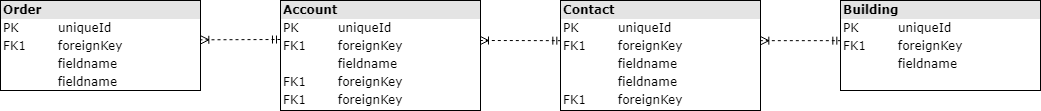
\includegraphics[width=12cm]{images/entityDiagram.png}
    \caption[Entity diagram of the CRM data]{Entity diagram for Contoso CRM data}
    \label{fig:entity-diagram}
\end{figure}

\subsection{Orders}\label{sec:crm-orders}

The \texttt{Order} entity holds all information about an order made by an account. Dynamics 365 contains all orders carried out by Contoso since 2013. In this project, all orders from January 2013 until June 2018, included, are considered. Once the raw data has been download, this set of 808'532 orders needs to be cleaned. Indeed, even if a CRM saves its data in an organized manner and that Dynamics 365 has some verification upon data entry, mistakes can still happen when a person enters data into the system. Orders have been discarded based on their names - empty or not -, on their status - active or not - and on their internal characteristics (amount delivered equal to zero, delivery date in 1956, delivery date occurring before the order date, ..). This cleaning phase removes 28.79\% of the orders, which gives a data set of 575'679 orders, each order having 37 features.

All these orders have been made by 183'706 accounts, with a mean of 3.14 orders per account and a median of 2. Grouping accounts per the number of orders reveals that 50.77\% of accounts have made only one or two orders\footnote{Accounts which have made at least one order since 2013.}. This demonstrates the singularity of a very competitive market in which clients often change their suppliers and fully benefit from the competition. In respect to the machine learning model, it will be very difficult to extract some common behavior and generalization out of these accounts. Therefore, accounts with less than three orders have been discarded, leading to a dataset composed of 451'986 orders (-21.49\%).

\begin{figure}[h]
    \centering
    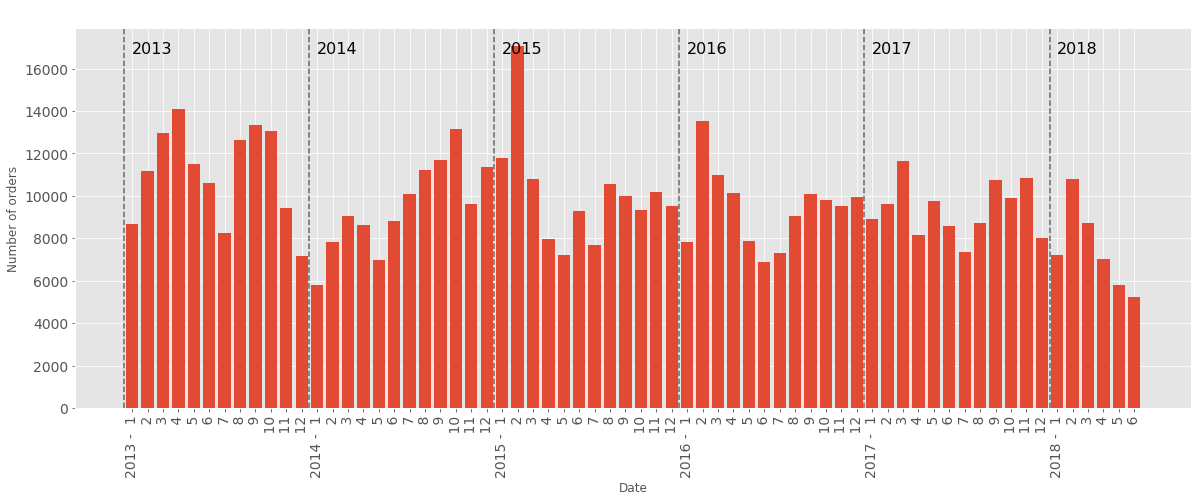
\includegraphics[width=15cm]{images/order_month_year.png}
    \caption{Number of orders per month per year}
    \label{fig:order_per_monthyear}
\end{figure}

Because \textit{normal} accounts only order once per year, there is a seasonality effect visible when plotting the number of orders per month through  the years (figure \ref{fig:order_per_monthyear}). Even if the periodicity of orders isn't regular, a year experiences two pics of orders: one around March and another around October. On the opposite side, there have been fewer orders in the Spring, around June. The data indicate that the weather must play a role when accounts are making orders - it's colder in March and October than in June. As detailed in \ref{sec:external-data}, the model will take some weather-related information into consideration.

Typical customer will make an order once per year, with a number of months between two orders around 12 months, A mean of 12.67 months and a median of 11 months are retrieved with the average \textit{wait} time between two orders for all accounts. Figure \ref{fig:orders-account-counts} shows that there are a lot of accounts waiting 11 months between two orders, but there are also accounts which order more frequently. On the other side, the number of accounts waiting 13 or more months between two orders decreases. Within this plot, there are two pics: the first one around 11 months and the second one around 23 months. This second pic is probably due to \textit{jumper accounts}, accounts that order one year with Contoso, the following year with the competition and, two years after their first order, order again with Contoso. 

\begin{figure}[h]
    \centering
    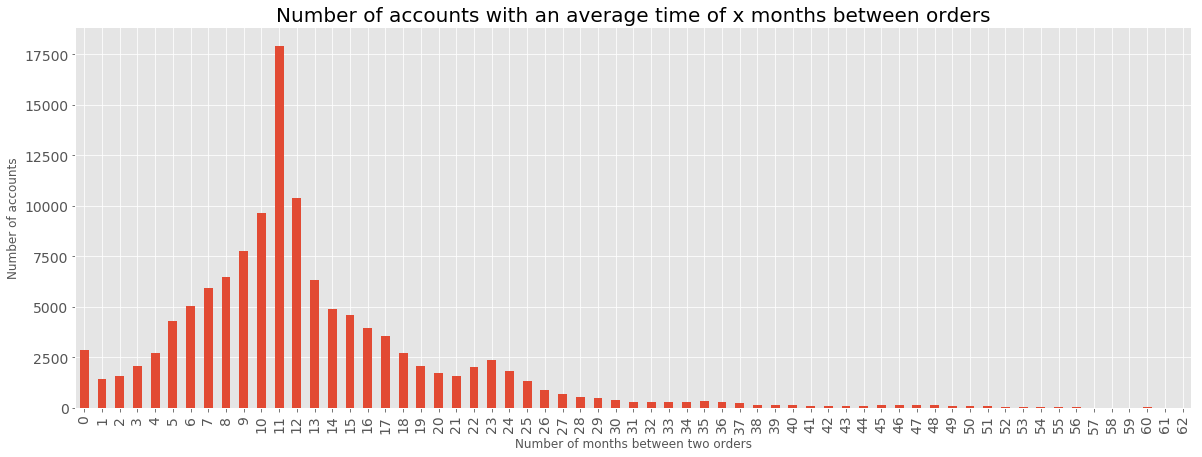
\includegraphics[width=15cm]{images/accounts-average-time-orders.png}
    \caption[Average number of months between two orders]{Accounts grouped by the average number of months between two orders}
    \label{fig:orders-account-counts}
\end{figure}

This plot also reveals \textit{key-accounts}, accounts ordering at least once per month. Those accounts are most of the time companies, considered as very regular customers by Contoso. As detailed in section \ref{sec:data-shape-for-ml}, \textit{key-accounts} will not be a problem for the machine learning model.


\subsection{Accounts, Clients and Buildings}\label{sec:crm-accounts}
The \texttt{Account} entity holds information related to the clients of Contoso, either a natural or legal person. Due to imports from a legacy system, the Dynamics 365 instance of Contoso contains more than 1'100'000 accounts. Filtering those accounts based on the final orders from section \ref{sec:crm-orders} reduces the set to 88'552 accounts, with 244 features per account. The company stocks a lot of properties for each account and the vast majority of these are null or not useful for the current task. After a review of all these features, only 11 will be kept, among which account's activeness and account's name. The name of the account is compared to the name of the primary contact.

Indeed, all accounts are linked to a primary contact. The \texttt{Contact} entity holds information about a physical person, like its address or phone number. From this entity, only two features are used: the birth date and the name. The birth date is used to evaluate the influence of a person's age on its buying habits. The contact's name is compared to the account's name. As mentioned above, the \texttt{Account} entity can be a natural or a legal person, but there is no feature in the CRM to specify this. As this information is important - a legal person can make orders on a very frequent basis - a feature is built to capture this notion. If both names are equal, the account is considered as a natural person, otherwise the account is considered as a legal person. The assumption is that an account modeling a legal person will not have the same name as it's primary contact (e.g. Account \textit{EPFL} linked to primary contact \textit{Martin Vetterli}). As shown in figure \ref{fig:account-contact-name-orders}, accounts classified as a legal person (in red) made orders much more frequently than \textit{person-accounts} (in blue).

\begin{figure}[h]
    \centering
    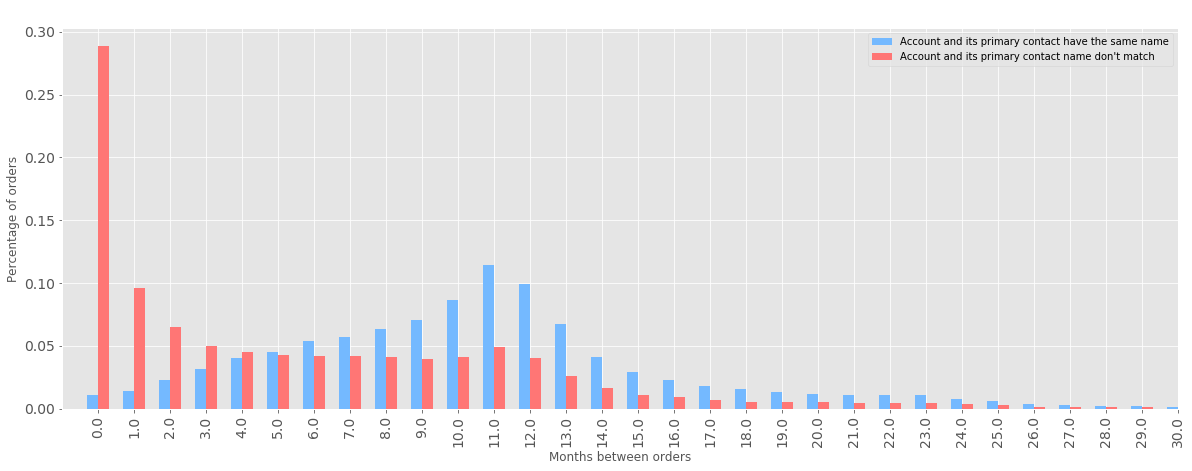
\includegraphics[width=15cm]{images/account-contact-name-orders.png}
    \caption[Account and contact's name influence of order's frequency]{Number of months between two orders related to the account-contact name}
    \label{fig:account-contact-name-orders}
\end{figure}

Regarding the \texttt{Reservoir} entity, it holds information about the reservoir of a building (house, offices, cottage, ...). Even if not all accounts have such link (19.16\% of accounts are not linked to any building), this entity is used to build new features to model the amount of product stocked and used, as detailed in section \ref{sec:ml-features}. The \texttt{Building} entity solely purpose is to \textit{link} accounts with reservoirs.

\subsection{External data}\label{sec:external-data}
In addition with the data coming from Dynamics 365, there are two important variables to take into account: price and weather. Two datasets have been created to encapsulate the price and the weather. Those datasets are then used to create new features in section \ref{sec:ml-features}.

As explained above, prices are mainly dependent on the stock market, which can change every day. It has been observed by Contoso that when the price is going down, more orders are coming in \footnote{In February 2015, then price went up after going down for seven consecutive months. In one year, the price dropped by 36.4\% so when it started to go up, people hurry to make orders. This pic of orders is visible in figure \ref{fig:order_per_monthyear}.} and when the price is going up, customers would rather hold, consume their stock and wait for a decrease in price to place a new order. A dataset containing the monthly prices of Contoso's product between 2012 and 2018 has been created. Unfortunately, it was not possible to compare this data with the monthly prices set by each competitor.

Weather data has also an influence on the ordering patterns of clients, as shown in section \ref{sec:crm-orders}. Weather data has been provided by \texttt{MeteoSwiss} with several daily metrics (weather, precipitations, wind, ...) associated to the 20 meteorological station across Switzerland. Based on the primary contact address, each \texttt{account} has been linked to one of those stations and among all metrics, only the weather degrees \big[°C\big] have been used.


\section{Data for the machine learning}
The data for all CRM's entities need to be shaped so that the machine learning models can make use of it. This section details how the data from \ref{sec:crm-data} has been combined and reshaped to be given to predictive models.

\subsection{Dataset construction}\label{sec:data-shape-for-ml}
As defined above, the model is planned to be used on a monthly basis and its output will be the number of months until customer's next order. For all accounts, one entry per month is created, from the month following client's first order until the month of last order. The output is the number of months until customer's next order. The data in these monthly entries contain features related to the account (shared among all entries), features related to the previous orders and features related to the current month, like the monthly weather for example. 

Figure \ref{fig:data-build-example} contains an example of the data creation process. This account has made four orders in April 2013, March 2014, January 2015 and March 2016, marked as yellow circles. The first entry in the data relates to May 2013, the month following account's first order. The output of this entry is set to 11 months, the number of months between May 2013 and March 2014, date of account's second order. The same principle is applied to all months, until March 2016, date of the last order made by this account.

\begin{figure}[h]
    \hspace{-1cm}
    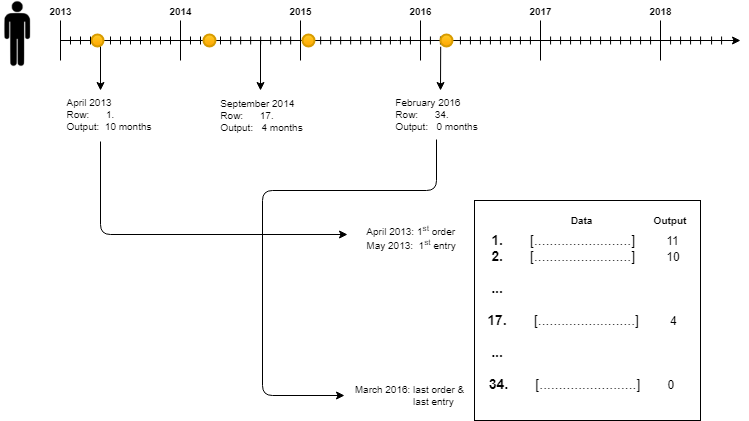
\includegraphics[width=17cm]{images/data-build-ml-example.png}
    \caption[Process to build data for machine learning]{Sketch of the process to build data for the machine learning models. Yellow circles model account's orders through time. The entry 1. corresponds to the month May 2013, the entry 17. to September 2014 and the entry 34. to March 2016.}
    \label{fig:data-build-example}
\end{figure}


% -------------------------------- Section: Customer Jounrey + Feature engineering
\subsection{Feature engineering}\label{sec:ml-features}

Before creating new features, all datasets must be combined together. Starting from right to left on figure \ref{fig:entity-diagram}, \texttt{Building} and \texttt{Reservoir} data are combined. If a \texttt{Building} is not linked to at least one \texttt{Reservoir}, it's discarded. Then the data is combined with the \texttt{Account} entity, a one-to-many relation (an account can be linked to one or more buildings). From \texttt{Building} and \texttt{Reservoir}, only one feature is used: the volume of its reservoir. In the case of multiple buildings being linked to the same account, the average capacity of all reservoirs is considered.

Then, the entities \texttt{Account} and \texttt{Contact} are combined based on the account's primary contact, with its address and birth date added to the account. This combination of \texttt{Account}, \texttt{Contact}, \texttt{Building} and \texttt{Reservoir} entities builds a first set of features, defined as \textit{account-related} features.

Each row in the final machine learning data is composed of three types of features: the \textit{account-related} ones, features related to the current month and features about the previous order. Features related to the current month are mainly built from the two external data to encapsulate the variations of price and weather temperature through time. Finally, some characteristics of account previous order are used, like "\textit{Was it a big or a small order}?" or "\textit{When did this order occurred compare to the one before?}".


\begin{figure}[h]
    \centering
    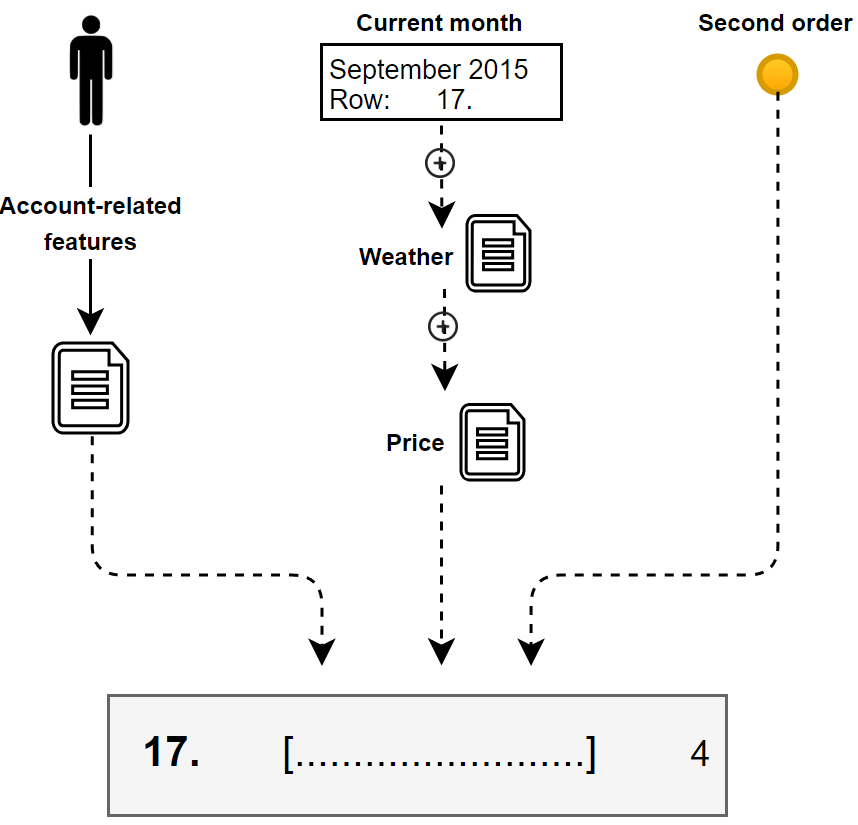
\includegraphics[width=8cm]{images/data-build-ml-example-row.png}
    \caption[Features building for specific month]{Sketch of the features used for the row of September 2014 in figure \ref{fig:data-build-example}}
    \label{fig:data-build-row-example}
\end{figure}

The exhaustive list of the 122 features built can be found in annex \ref{annex:features-for-ml}. Those features are based on Contoso's knowledge of its business, but also on analyses of \textit{Customer Journeys}. A \textit{Customer Journey} is a plot where all orders of a given account are visible, with the \texttt{Weather} and \texttt{Price} information over time (see an example in figure \ref{fig-annex:customer-journey}). \textit{Customer Journeys} have been used as a starting point to understand the order's pattern of accounts, the influence of external data and the general behavior of Contoso's clients.

Some features have also been created after a trial and error phase while building and testing machine learning models. The property \texttt{feature\_importances\_} of \textit{Sklearn}'s models has also been used to rank features and build new ones based on it.



% -------------------------------- Section: Machine Learning Experimentation
\section{Machine Learning Experimentation} \label{sec:ml-experimentation}

It is the first time Contoso is involved in a machine learning project with the goal to model its customer's behavior. Therefore, all types of models and architectures are possible. In this project, it has been decided to start with several types of models and a simple set of features. The first goal is to evaluate the feasibility of the task and the family of machine learning models best suited for it. 


\subsection{Models experiments}
Python' package \textit{Scikit-learn} was used to build the models of this section. Scikit-learn enables to test different models very easily and based on it, several families of supervised learning models have been investigated, with the results reported in table \ref{tab:scores-simple-models}. Among the models investigated, there are \texttt{Liner models} (linear regression), \texttt{Tree models} (extra tree and decision tree), \texttt{Ensemble models} (random forest, extra trees, and bagging regressor) and \texttt{Neighbors models} (kneighbors regressor).

In this initial phase, all models have been trained with scikit-learn's default parameters and a subset of 17 features manually selected\footnote{Those features are marked with an * in annex \ref{annex:features-for-ml}.}. For all models created, the random number generator has been seed.

\begin{table}[htb]
    \begin{tabular}{l|ccc|ccc}
                          & \multicolumn{3}{c|}{Train}                         & \multicolumn{3}{c}{Test}      \\
        \textbf{Model name}        & \textbf{Precision} & \textbf{Recall} & \textbf{F1-score} & \textbf{Precision} & \textbf{Recall} & \textbf{F1-score} \\ \hline
        Extra Tree        & 0.996     & 0.999  & 0.998                         & 0.324     & 0.389  & 0.354    \\
        Decision Tree     & 0.996     & 0.999  & 0.997                         & 0.267     & 0.394  & 0.318   \\
        KNeighbors        & 0.303     & 0.908  & 0.455                         & 0.131     & 0.508  & 0.208    \\
        Random Forest     & 0.696     & 0.998  & 0.820                         & 0.046     & 0.829  & 0.088    \\
        Bagging Regressor & 0.699     & 0.998  & 0.822                         & 0.045     & 0.829  & 0.084    \\
        ExtraTrees        & 0.996     & 0.999  & 0.998                         & 0.044     & 0.829  & 0.083    \\
        Linear Regression & 0.011     & 0.187  & 0.021                         & 0.028     & 0.305  & 0.051    
    \end{tabular}
    \caption[Prediction scores for first models]{Prediction scores for first models, ranked by their F1-score on the testing set}
    \label{tab:scores-simple-models}
\end{table}

The first observation is that F1-scores aren't high and more than half of the models have a score below 0.10. It's also noticeable that all models are overfitting too much, except for the linear regression which has difficulties to combine the 17 features. The two tree models are giving the best predictions, with a good trade-off between precision and recall. The ensemble models are very confident in their predictions (recall score above 80\%), but too cautious and catch less than 5\% of the orders.

The next experiments are related to the set of features used. With the \texttt{Extra Tree} models, three features selection techniques have been used: Univariate selection where features are scored with the \textit{f\_regression}, Principal Component Analysis (PCA) and feature importance based on an \textit{ExtraTrees} model. The best F1-score turned out to be obtained with six features, selected by the \textit{ExtraTrees} model. With a F1-score of \texttt{0.636}, the model trained with only six features achieves a score almost twice as good as the one obtained previously. It's clear that this model gives it's better predictions when using a small number of features, as reported in figure \ref{fig:feature-selection}.

\begin{figure}[htbp]
    \centering
    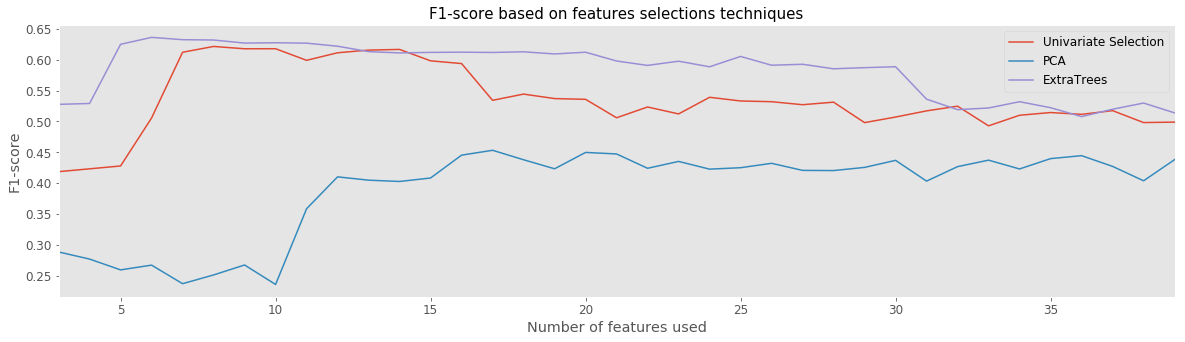
\includegraphics[width=15cm]{images/feature_selection.png}
    \caption[F1-score based on feature selection]{F1-score obtain on the testing set with three different strategies for features selection.}
    \label{fig:feature-selection}
\end{figure}


After optimizing the set of features, \textit{ExtraTree} regressor's internals parameters can also be optimized. The primary goal is to reduce the overfitting affecting tree models. Two parameters have been optimized: \texttt{max\_depth} and \texttt{min\_samples\_split}. The \texttt{max\_depth} parameter has no value by default, therefore the tree expands itself until all leaves are pure. The \texttt{min\_samples\_split} parameter controls the minimum number of samples required for a node to be split. By default, \textit{ExtraTree} splits all nodes as soon as possible, when it contains two samples. This default splitting strategy combined with unlimited depth explains the overfitting obtain on the training data.

The most relevant results of this optimization phase are reported in table \ref{tab:tree-fine-tune}. With the best combination of \texttt{max\_depth} and \texttt{min\_samples\_split}, the model reaches an F1-score of 0.715 on the testing data. Results also show that the model is not overfitting anymore, with similar results on the training data. Regarding the two parameters investigates, \texttt{min\_samples\_split} has more impact on the predictions that \texttt{max\_depth}. Results show that the tree will not expand itself after 50 depth levels (same scores if the parameter is set to 50 or 80). Overfitting on the training data happens when the tree splits its nodes \textit{too early}, with a small number of samples inside them.


\begin{table}[htbp]
    \centering
    \begin{tabular}{c|c|c|c}
    \textbf{Max depth} & \textbf{Min samples split} & \textbf{Training F1-score} & \textbf{Testing F1-score} \\ \hline
    30	&  70   &  	0.738  &  0.715 \\
    50	&  100  &  	0.729  &  0.713 \\
    80	&  100  &  	0.729  &  0.713 \\
    30	&  100  &  	0.730  &  0.711 \\
    30	&  50   &  	0.748  &  0.710 \\
    50	&  70   &  	0.739  &  0.710 \\
    80	&  70   &  	0.739  &  0.710 \\
    50	&  50   &  	0.749  &  0.707 \\
    80	&  50   &  	0.749  &  0.707 \\
    30	&  10   &  	0.828  &  0.696 \\
    50	&  10   &  	0.854  &  0.683 \\
    80	&  10   &  	0.854  &  0.683 \\
    10	&  100  &  	0.449  &  0.466 \\
    10	&  10   &  	0.470  &  0.396 \\
    10	&  50   &  	0.439  &  0.388 \\
    10	&  70   &  	0.378  &  0.364 
    \end{tabular}
    \caption[F1-scores for ExtraTree hyperparameters optimization]{F1-scores on training and testing data for the hyperparameters optimization phase. Parameters investigated are the \texttt{max\_depth} and \texttt{min\_samples\_split}. Models trained on a set of six features previously selected. Table sorted by decreasing score on the testing set.}
    \label{tab:tree-fine-tune}
\end{table}

Alongside with experimenting models and new parameters, optimizing the data used to train models is examined. In previous experiments, data-related optimizations have only concern the features set, but there are some others possibilities. By investigating the data, three possible ways to reshape it are found. 
The first one consist of reducing the data by removing accounts with less than five entries. Then, for the remaining accounts, only five random entries are selected. The goal is to reduce the potential influence of accounts ordering very often but also the potential noise generated by accounts with very few entries, for example an account with four orders spread across five months. A second attempt to reduce the influence of \textit{extreme} accounts is to simply remove all accounts ordering every month or every two months. The third and last experiment to reshape the data is to have the same number of entries per output. These three attempts to reshape the data never improved the F1-score previously obtained.

To summarize this section about experimenting with several models, the best model is an \textit{ExtraTree} regressor trained on a small set of features. After an hyperparameters optimization phase, it achieves a F1-score of 0.715 on the testing dataset, a precision score of 0.813 and a recall score of 0.638.


\subsection{Neural Networks}
The \textit{ExtraTree} model has a big flaw: it's only using six features and none about the weather nor product's price. When adding these kind of features, the predictions aren't as good as before. Therefore, a new type of machine learning model is investigated: \textit{Neural Networks}. Build with the \textit{Keras} framework, six different architectures of neural networks are experimented, all based on fully-connected layers. Similar to what has been done with previous models, several sets of manually selected features are used. The best model has a complete architecture composed of five fully-connected hidden layers trained with a set of 23 features and reached an F1-score of \texttt{0.820} on the test data. Details, results, and analysis of all tested models are reported in annex \ref{annex:nn-experiments}.

Once the model's architecture is chosen, internal parameters can be investigated. Four parameters deserve some attention: the training \texttt{batch size}, model's compiler \texttt{loss function} and \texttt{optimizer} and the hidden layers \texttt{activation} function. Due to all possible values for those parameters, an hyperparameter grid-search phase is done sequentially: starting from the best model in table \ref{tab-annex:nn-experiments}, optimize the training batch size, then the activation function of hidden layers, the model's compiler loss function and finally the model's optimizer function (results reported in annex \ref{annex:nn-fine-tuning}). The best parameters obtained are outlined in table \ref{tab:nn-final-parameters}.

\begin{table}[h]
    \centering
    \begin{tabular}{l|l|l}
        \textbf{Model part}           & \textbf{Parameter}                 & \textbf{Value}         \\ \hline
        Training                      & Number of epochs                   & 4                     \\
                                      & Batch size                         & 70             \\
                                      & Input dimension                    & (nbr of samples, 23)                     \\ \hline
        Hidden layers                 & Number of neurons                  & 200-150-90-60-30                     \\
                                      & Activation function                & elu                     \\
                                      & Use bias                           & Yes                     \\ \hline
        Compiler                      & Loss function                      & log cosh \\
                                      & Optimizer                          & adam
    \end{tabular}
    \caption{Neural Network parameters for training final model}
    \label{tab:nn-final-parameters}
\end{table}


\subsection{LSTM}
A flaw present in previous models, neural networks included, is that the models are not account-specific. Despite the presence of some account-specific features, not all use cases can be caught. Let's assume that an account has a specific ordering strategy: make a big order in June, then make a smaller order as soon as the prices go down, for example in September, and repeat the same ordering strategy every 15 months. For such account, the previous model will most probably not be able to catch this behavior with the features used. That's the main motivation for considering \textit{Long Short-Term Memory} (LSTM) networks for this task. Being part of the Recurrent Neural Networks (RNN) family, LSTMs have the ability to recognize patterns in sequences of data. This is a different problem compared to other types of supervised learning since sequences impose an order on observations.

To be able to use LSTMs, the data need to be reshaped. Previous models were expecting a two-dimension input, but LSTMs requires data to be in a three-dimensions form: \texttt{[batch size, time steps, features size]}. To reshape the data, all entries related to the same account are sorted by month and year. Among all these entries, one is taken randomly and is considered as the last \textit{step} of the LSTM data, while all entries occurring before are considered as previous steps. Figure \ref{fig:lst-data-build} outlines this process. In order to have a dataset that a computer can still handle, the LSTM data is composed of a maximum of three entries per account and each entry has a maximum of 15 steps (15 monthly data).

\begin{figure}[htbp]
    \centering
    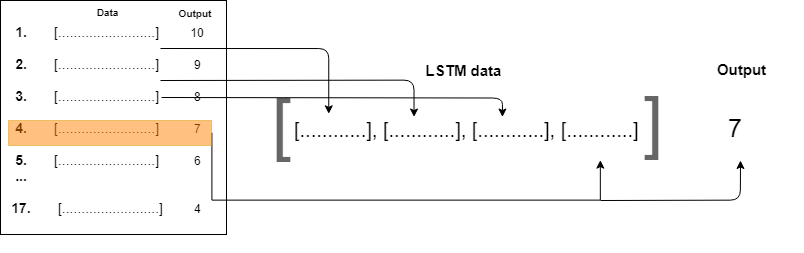
\includegraphics[width=10cm]{images/lstm-data-build.png}
    \caption[LSTM data build]{Example of reshaping the data for LSTM models. From the initial data, the fourth entry is randomly selected and placed as the last step of the data. Its output is the output for this data entrie. Orders 1, 2, and 3 are added as the first stepd of the data. All other orders are discarded.}
    \label{fig:lst-data-build}
\end{figure}

Similar to the experiments with previous neural networks, several model architectures are investigated to train LSTMs: one with only the LSTM layer, others with some fully-connected dense layers after the LSTM part. The results are available in annex \ref{annex:lstm-experiments}. LSTM models achieve F1-score close to the ones obtaines with previous models, but they are not better and have a longer training time.



\subsection{Best model evaluation}
\label{sec:best-model}

The best model is a Neural Network composed of five fully connected hidden layers with 200, 150, 90, 60 and 30 neurons. Trained with the parameters reported in table \ref{tab:nn-final-parameters}, it achieves the following scores:

\noindent\hspace*{0.8cm}  1. \texttt{Training data}:   F1-score of \textbf{0.784}, precision of 0.741 and recall of 0.833 \\
\hspace*{0.8cm}           2. \texttt{Testing data}:    F1-score of \textbf{0.823}, precision of 0.804 and recall of 0.843 \\
\hspace*{0.8cm}           3. \texttt{Validation data}: F1-score of \textbf{0.820}, precision of 0.750 and recall of 0.906

Since the task is scored with metrics used for classification problem, the confusion matrix obtain with the validation data is generated in figure \ref{fig:cf-matrix-validation}.

\begin{figure}[htbp]
    \centering
    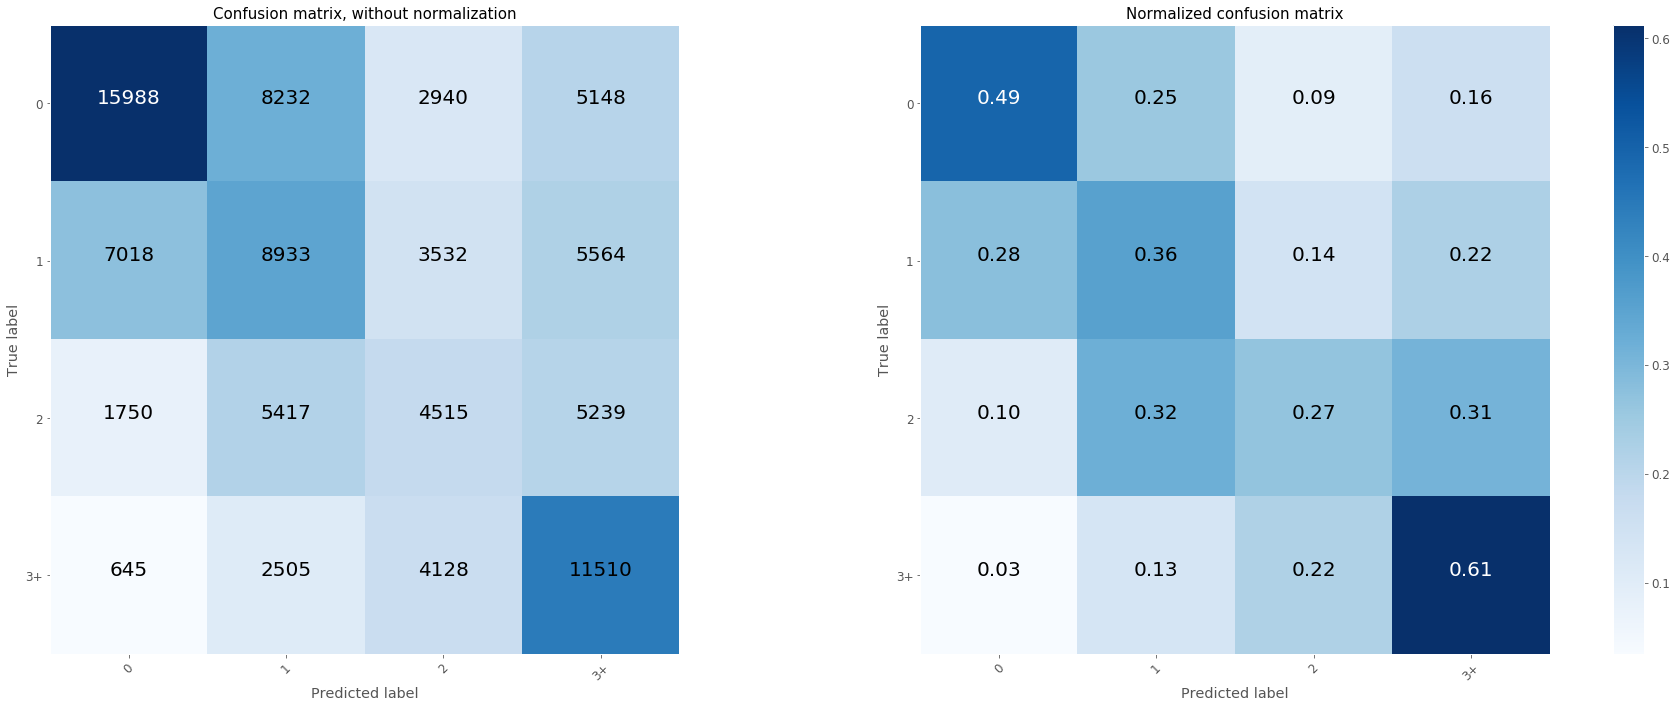
\includegraphics[width=15cm]{images/cf-matrix-validation_complete.png}
    \caption[Confusion matrix for validation data]{Confusion matrices for the validation data obtain with the best model. Two version: pure counts (left) and normalized per row (right).}
    \label{fig:cf-matrix-validation}
\end{figure}

Regarding the validation data, when an account makes an order, the model predicts it at the correct month-level almost one time out of two and one time out of four the model predicts it one month later. This gives a precision of 75\% with one month-tolerance. Among the predictions made by the model, 62.94\% of the predictions are correct at the month-level while 27.63\% are wrong for one month. Regarding the errors, most of them are wrong for two months (6.89\%) and only 2.54\% of the predictions are completely wrong. This seems to indicate that the model makes robust predictions.

By analyzing the errors, it emerges that in 40\% of the cases the predictions are wrong of two months and in 22\% wrong of three months. This means that a slight improvement on the model can potentially result in much more precise and trustworthy results. Error analysis also indicates that the model can sometimes be wrong for more than 40 months. This is due to \textit{inactive accounts}, clients who used to order, never order more for quite some time and order again. By classifying an account as \textit{inactive} if it hasn't made an order in the last 22 months, 8.09\% of the errors would have been avoid.

Analyzing the \textit{customer journeys} of wrongly predicted accounts reveals that some orders are simply impossible to predict and doesn't follow a pattern. But it also shows that the model could be improved by giving more weight and importance to the previous order. This is particularly true for jumper accounts, clients that made a order at year \textit{y, y+2,} and \textit{y+3}. The assumption is that these clients ordered from a competitor at year \textit{y+1}, but the model is not able to realize that the client \textit{skipped} one order and will give wrong predictions for the order at year \textit{y+3}.

% -------------------------------- Section: Deployment
\section{Deployment} \label{sec:crm-deployment}
With the final machine learning model build and tested, its results must be integrated within the Dynamics 365 instance of Contoso. The end goal is to have a prediction for each account regarding the date of its next order. For this, two ways to make account predictions are defined:
\begin{enumerate}
    \item Run the predictions every first Saturday for every month.
    \item Run the predictions for a specific account directly for the CRM interface, at anytime.
\end{enumerate}

Both integration are supported by \textit{Azure} services.

\subsection{Azure Architecture}
To deploy the model, four Azure services are used: \textit{Functions}, \textit{Queue Storage}, \textit{Web App} and \textit{Application Insights}. Azure Functions run a piece of code on a serverless architecture and can be scaled on demand. The Azure Queue Storage is a service to store large number of messages, which can be consumed via HTTP calls at a later stage. Azure Web App creates web application with built-in autoscale and Azure Applications Insights are used to analyze performances, errors and logs messages. The connection between those services and Dynamics 365 are sketched in figure \ref{fig:azure-deployment}.

\begin{figure}[htbp]
    \centering
    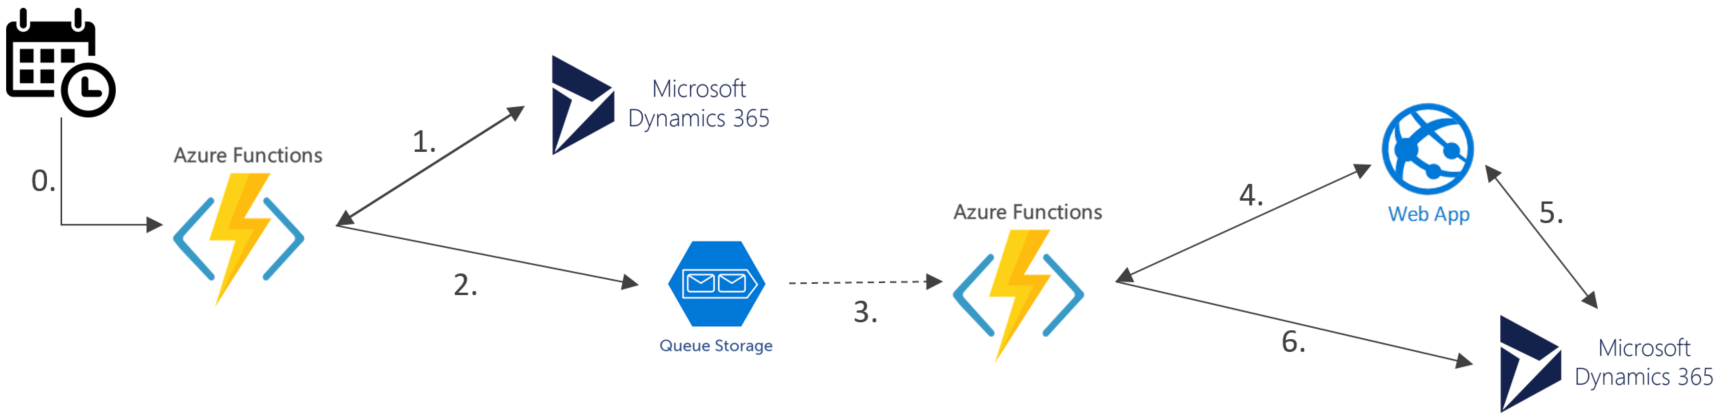
\includegraphics[width=12cm]{images/azure-archi-weekly.png}
    \caption[Deployment architecture for scheduled predictions]{Connection between Azure services and Dynamics 365 to compute predictions on a recurring basis.}
    \label{fig:azure-deployment}
\end{figure}

The architecture used to integrate machine learning predictions inside Dynamics 365 contains the following steps:
\vspace*{-\baselineskip}
\begin{enumerate}[label=\texttt{\arabic*.}]
    \setcounter{enumi}{-1}
    \item The first Saturday of each month, at 03:00, the entire process is triggered.
    \item A first Azure Function retrieves all accounts of interest in Dynamics 365, via the Web API. Only active accounts with at least three orders are retrieved.
    \item Once all accounts are retrieved, they are added into a queue stored as an Azure Queue Storage.
    \item A second Azure Function is triggered each time new items are added into the Azure Queue Storage. This function will process five accounts per run.
    \item The Azure Function retrieves the predictions for the five accounts with an HTTP call to the Web App.
    \item The Web App holds the entire logic of the predictions. When the Web App receives accounts one one of its HTTP endpoints, it connects to the CRM to retrieve and build the data for the machine learning. The ML model is stored in the Web App and used with the data just created. Predictions are then returned to the Azure Function.
    \item Once the Azure Function gets the predictions, it updates the CRM.
\end{enumerate}

One advantage of using this architecture is the connection between the Azure Queue Storage and the second Azure Function. It enables accounts to be consumed at a desired pace, in such a way to not overload the others components (Web App and Dynamics 365), to make the predictions before reaching the built-in timeout of Azure Functions, and to have another queue gathering failures. In case of an error during the process, accounts for which the predictions weren't computed are added to this \textit{failure queue}, in such way that they do not stop the entire process. Through all steps, Azure Application Insights are used to store logs.

Experiments with this architecture showed a total running time of approximately 8 hours for 106'000 accounts. Compared to others services powered by Azure like the \textit{Azure Machine Learning}'s suite, this architecture is significantly less expensive, much more flexible and better suited for this use case where data is created on-the-fly.

The Azure Web App described above is also used to run the prediction for a specific account, upon CRM's user request. In that case, Dynamics 365 sends an HTTP request to the Web App and updates the \textit{Account} entity.

\subsection{Integration with Dynamics 365}
The predictions made by the machine learning model must be visible and usable directly from Dynamics 365. Inside the \texttt{Account} entity page, a section \texttt{ML Predictions} is created with two fields: \texttt{Next Order Prediction} and \texttt{Last refresh}. An example of such page is visible in figure \ref{fig:dynamics-account-ml-screenshot}. The first field contains the predicted month for account's next order. The date the machine learning model was ran is displayed below, in the second field. This enables CRM's users to see the prediction and when it was made. If the prediction is \textit{too old} or that new account-related information has been added to Dynamics 365, predictions can be refreshed on-demand with the blue button \texttt{Run predictions}. This button is grayed out and inactive throughout the entire process (approx. 5-10 seconds). No refresh or page reload is necessary, both fields are automatically updated. If the process ends successfully, the button turns out green, but if a mistake happens, the button is red.

\begin{figure}[!htb]
    \centering
    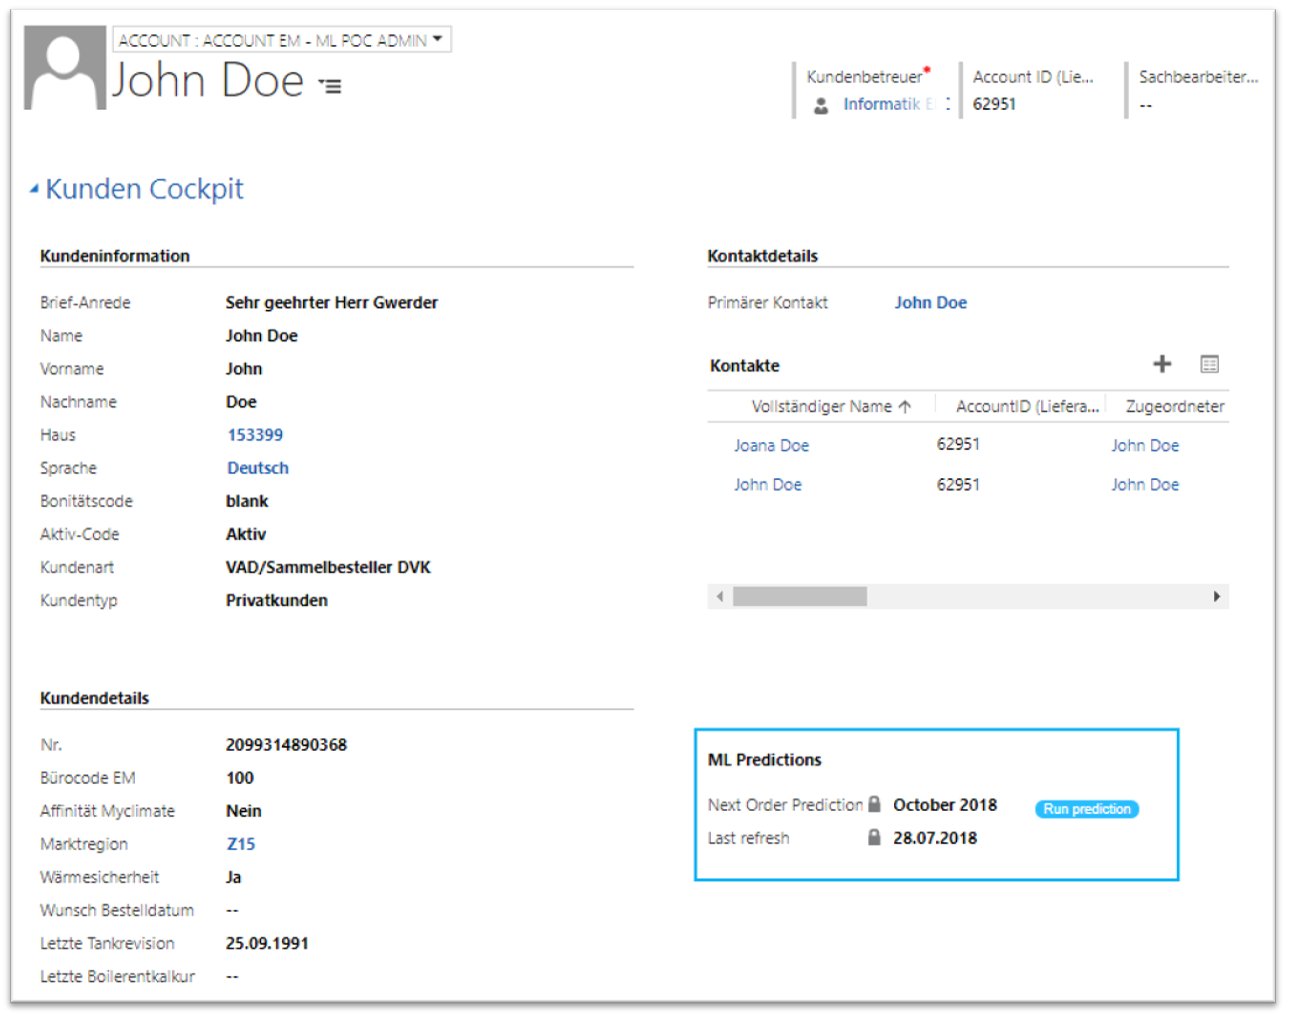
\includegraphics[width=12cm]{images/dynamics-account-ml-screenshot.png}
    \caption[Dynamics 365 \textit{Account} entity page]{Dynamics 365 Account entity page. The part related to the machine learning prediction is in the blue rectangle. It contains two fields: \texttt{Next Order Prediction} and \texttt{Last refresh}, as well as a button \texttt{Run prediction}.}
    \label{fig:dynamics-account-ml-screenshot}
\end{figure}

Predictions are stored as a CRM field and can be used to create \textit{Marketing lists}. In Dynamics 365, creating a marketing list is usually the first step in a marketing campaign. For Contoso's use case, a marketing list can contain all accounts with the field \textit{Next Order Prediction} happening in the current or coming month. Then, those accounts can be contacted before they make an order and investigate competitor's offers.


% -------------------------------- Section: Further Work
\section{Discussion} \label{sec:use-case-further-work}
The models built for this task rely heavily on feature engineering. Indeed, data coming from CRM needs to be combined and reshaped to bring useful value to a machine learning model. The set of features used with the best model is not giving a lot of importance to the \textit{external} data: weather and price-related features. Based on the customer journey visualization and Contoso's business knowledge, these two external factors play a role in the customer's ordering pattern. New features or even new models can be investigated to incorporate such information.

A possible method to improve current models is to include features related to the customer's profile, for example customer's price sensitivity. Such features would help the model to weight the importance of price-related information. It will also enable Contoso to make personalized offers to customers. For example, if a customer is flagged as a \textit{jumper profile} with high price sensitivity, a personalized offer can be proposed to retain the customer.

The last phase of this project involves the deployment and integration of a machine learning model within a Dynamics 365 instance. The architecture is built for the current Contoso's usage of predictions: monthly usage of predictions with no time constraints to make them. If the company decides to change the way of working with the predictions, to run them once or twice per week, the current architecture might not be adequate. The cloud-based components of Azure can be scaled, but creating data on-the-fly is a time-consuming step. Having part of the data static (account-related features) and only build the month-related features like the "\textit{number of weeks since last order}" or "\textit{weather of past week}" is an interesting option.

In the literature, the vast majority of machine learning projects involving customer data concern the "market basket analysis" task. It's a problem where customers have a purchase history with several products through time \cite{temporal-feature}. Contoso's use case is more related to event predictions tasks for rare events \cite{7953302, Malhotra2015LongST}, but modeling repeat purchasing patterns and not only one-time occurrence. Further work on this problem can draw inspiration from other research fields like bio-medical studies for recurrent events \cite{biomedical-recurrent-events} or e-commerce related studies \cite{Liu:2016-repeat-buyer, Tian2015}. 

Nevertheless, neural networks are used in the majority of recent studies. A drawback of using a neural network model compared to linear or tree-based model is that there are no justifications for the predictions. CRM users have access to the predictions, but there is no feedback or explanation \textit{why} the neural network outputs such prediction.

Regarding the LSTM neural networks, it's an interesting option if Contoso's decided to change the scoring strategy. For example, if the number of weeks until next order are predicted instead of the number of months, LSTMs might give better predictions than a fully-connected network. Indeed, the LSTM models built had a better $t_0\_p_0$ score compared to other models. The assumption is that LSTM models are more robust and confident regarding the \textit{closest} predictions.

% -------------------------------- Section: Conclusion
\section{Conclusion} \label{sec:use-case-conclusion}
In this project, real-world data coming from a CRM are used to create predictions regarding the date of the next customer order. Predictions are given by a neural network composed of five fully connected layers. Trained with all orders between 2013 and 2016, the model reaches an F1-score of 0.828 for 2018 orders. The F1-score used is a harmonic mean between the precision and recall of the model, two metrics computed with one-month tolerance on predictions.

An Azure-based architecture supports the incorporation of the predictions into the daily usage of Dynamics 365. This architecture enables recurrent predictions with user-intervention, as well as one-demand prediction requested directly by Dynamics 365 users.